\documentclass[12pt]{article}
\usepackage[utf8]{inputenc}
\usepackage{listingsutf8}
\usepackage{color} 
\usepackage{graphicx}
\usepackage{geometry}
\geometry{a4paper,left=2.5cm, right = 2cm , top= 3cm, bottom = 3cm}
\setlength{\parindent}{0cm}
\definecolor{codegreen}{rgb}{0,0.6,0}
\definecolor{codegray}{rgb}{0.5,0.5,0.5}
\definecolor{codepurple}{rgb}{0.58,0,0.82}
\definecolor{backcolour}{rgb}{0.9,0.90,0.84} 
\lstdefinestyle{mystyle}{
    backgroundcolor=\color{white},   
    commentstyle=\color{codegreen},
    keywordstyle=\color{blue},
    numberstyle=\tiny\color{codegray},
    stringstyle=\color{codepurple},
    basicstyle=\footnotesize,
    breakatwhitespace=false,         
    breaklines=true,                 
    captionpos=b,                    
    keepspaces=true,                 
    %este comando sirve para habilitar la presencia de la linea de numeros
    numbers=left,                        
    numbersep=5pt,                  
    showspaces=false,                
    showstringspaces=false,
    showtabs=false,                  
    tabsize=2
}
 
\lstset{style=mystyle}
\usepackage{fancyhdr}
\pagestyle{fancy}
\fancyhead{
\lhead{UMSA}
\chead{lab-111 E}
\rhead{Informática}
}											% No page header
\fancyfoot[L]{Marco Antonio Vino}											% Empty 
\fancyfoot[C]{}											% Empty
\fancyfoot[R]{\thepage}									% Pagenumbering
\renewcommand{\headrulewidth}{1pt}			% Remove header underlines
\renewcommand{\footrulewidth}{0.5pt}				% Remove footer underlines
\setlength{\headheight}{5pt}




%%% Maketitle metadata
\newcommand{\horrule}[1]{\rule{\linewidth}{#1}} 	% Horizontal rule

\title{
		%\vspace{-1in} 	
		\usefont{OT1}{bch}{b}{n}
		\normalfont \normalsize \textsc{Universidad Mayor de San Andres \\
        Facultad de Ciencias Puras y Naturales\\
        Carrera de Informática \\
        lab-111 E \\
        Lic. Jhonny Felipez Andrade} \\ [25pt]
		\horrule{0.5pt} \\[0.2cm]
		\huge Laboratorio \# 2 \\
       \horrule{2pt} \\[0.1cm]
}

\author{
		\normalfont 								\normalsize
        Marco Antonio Vino Chipana	 \\
        CI 9111299 L.P.\\[-3pt]		\normalsize
        \today
}
\date{}
\begin{document}

%\begin{center}
%\maketitle
 
%\section*{Práctica \#1 \\ Comandos para manejo de directorios, archivos y permisos}
%\end{center}
\maketitle 
\thispagestyle{empty}

\newpage

\textbf{1. Triángulo.} Escriba un programa que realice los cálculos sobre un triángulo,
x1, y1 
x2, y2 
x3, y3 \\
El trabajo consiste en calcular las siguientes propiedades del triángulo:\\
a)Las longitudes de sus 3 lados\\
b)Los ángulos de las 3 esquinas\\
c)El perímetro\\
d) El área 


\textit{Diagrama de Flujo:  }
\begin{figure}[h!]
\centering
	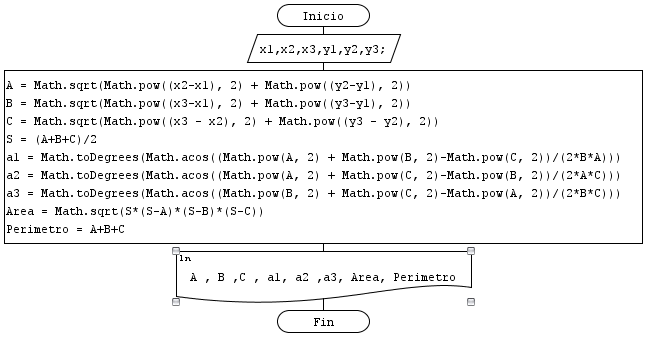
\includegraphics[scale=0.65]{dicor/Triangulo.png}    
\end{figure}

\textit{Código en Java:}
\lstinputlisting[language = Java]{src/Triangulo.txt}
\newpage



\textbf{2. Intervalo.} Escriba un programa que lea dos hora e imprima el número de horas y minutos entre estas 2 horas.  
\textit{Diagrama de Flujo:  }
\begin{figure}[h!]
\centering
	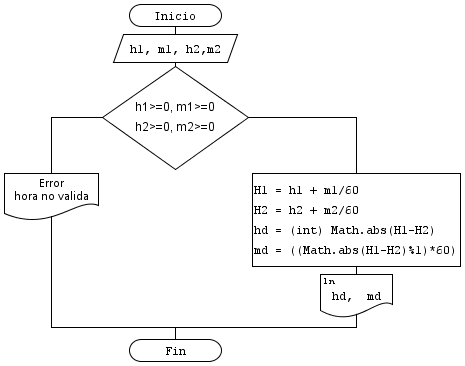
\includegraphics[scale=0.6]{dicor/Intervalo.png}    
\end{figure}

\textit{Código en Java:}
\lstinputlisting[language = Java]{src/Intervalo.txt}
\newpage



\textbf{3. Conversión.} Escriba un programa para convertir un valor, de una unidad en otra unidad 
de distancia. Las unidades se encuentran en m(i)límetros, (c)entímetros, (m)etros y
(k)ilómetros. Lea las dos unidades y luego el valor dado. Ejemplo:
Convertir de: i
Convertir a: c
Valor: 10
10 milímetros = 1 centímetro.

\textit{Diagrama de Flujo:  }
\begin{figure}[h!]
\centering
	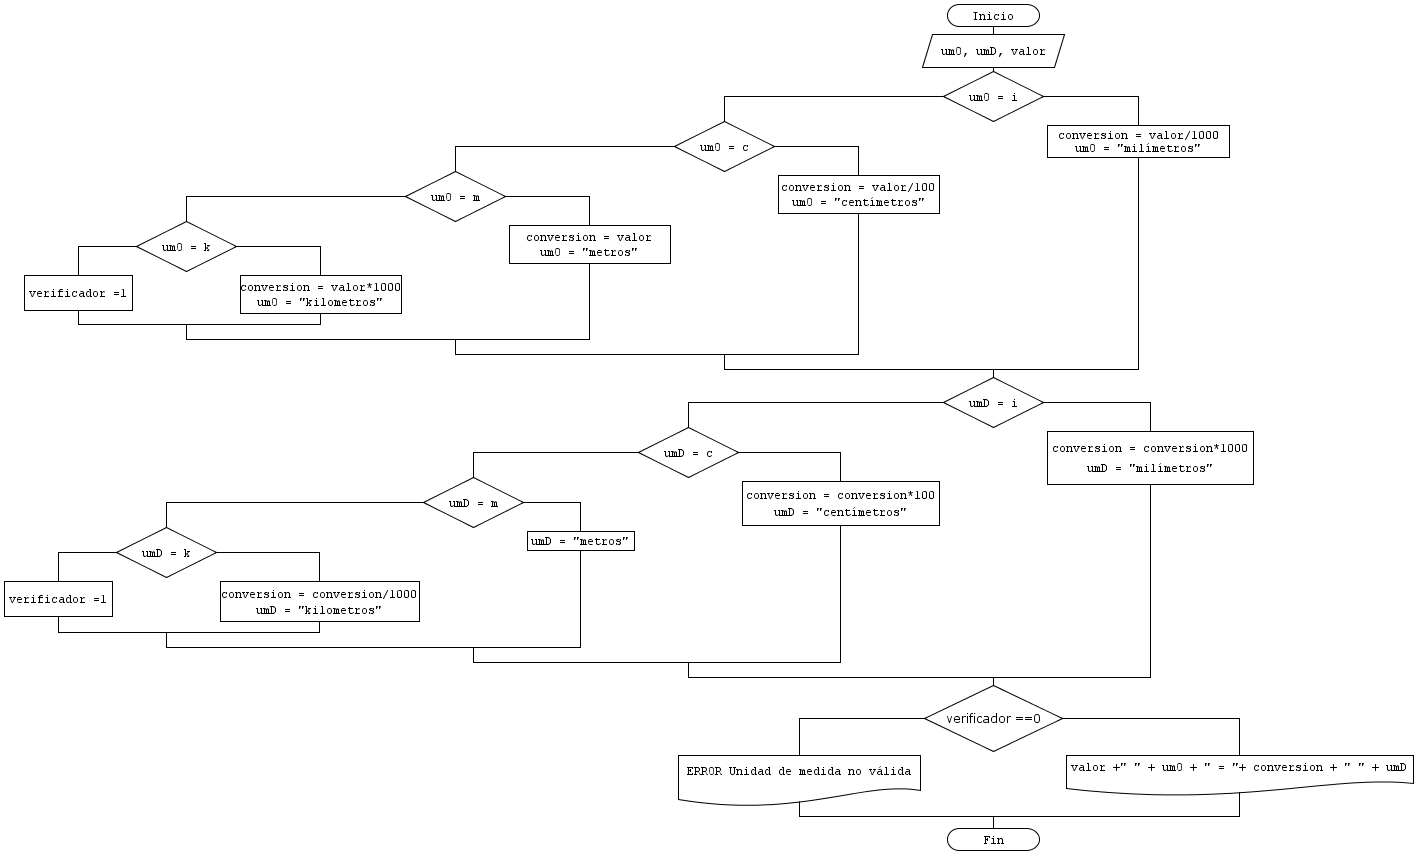
\includegraphics[scale=0.35]{dicor/Conversion.png}    
\end{figure}

\textit{Código en Java:}
\lstinputlisting[language = Java]{src/Conversion.txt}
\newpage


\textbf{4. Ordena 3 números.}  Leer 3 números e imprimir de manera ascendente.  

\textit{Diagrama de Flujo:  }
\begin{figure}[h!]
\centering
	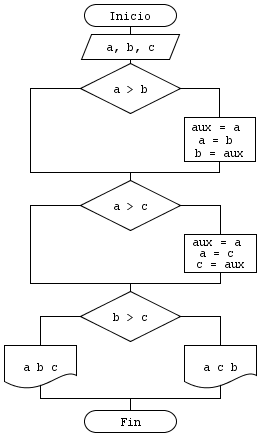
\includegraphics[scale=0.85]{dicor/OrdenaTresNumeros.png}    
\end{figure}

\textit{Código en Java:}
\lstinputlisting[language = Java]{src/OrdenaTresNumeros.txt}
\newpage


\textbf{5. Logaritmo.} Escriba un programa java que lea la base b (entero) y el número x (real).
Imprima el resultado del logb x. Valide si x es negativo:
Ejemplo de entrada; \\
base = 2 
x = 0.5\\
Ejemplo de salida\\
-1

\textit{Diagrama de Flujo:  }
\begin{figure}[h!]
\centering
	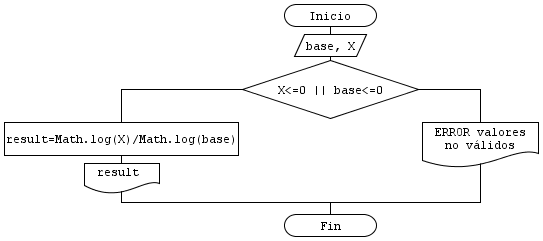
\includegraphics[scale=0.70]{dicor/Logaritmo.png}    
\end{figure}

\textit{Código en Java:}
\lstinputlisting[language = Java]{src/Logaritmo.txt}
\newpage


\textbf{6. Verifica.} Verifíque con un programa si son cierta las siguientes identidades, donde a, b y
c son las longitudes de los lados de un triángulo. A, B y C son los ángulos opuestos a los
lados respectivamente:

\textit{Diagrama de Flujo:  }
\begin{figure}[h!]
\centering
	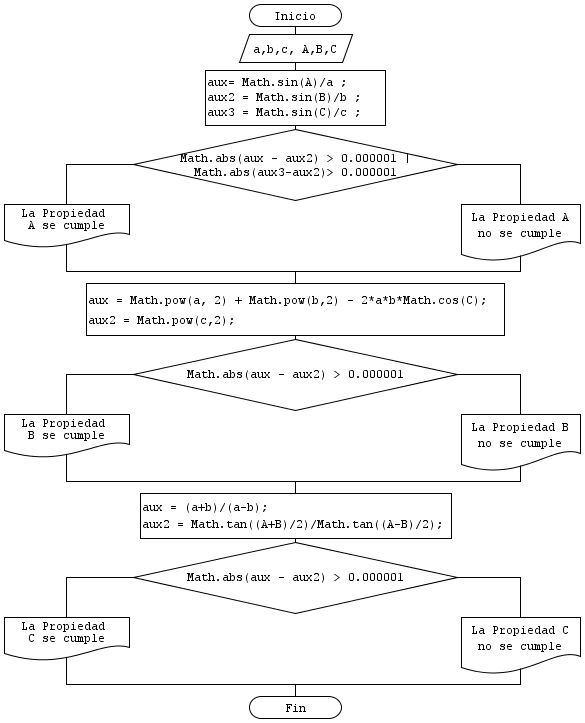
\includegraphics[scale=0.80]{dicor/Verifica.png}    
\end{figure}

\textit{Código en Java:}
\lstinputlisting[language = Java]{src/verifica.txt}
\newpage

\textbf{7. Verifíca.} Verifíque con un programa si son cierta las siguientes propiedades de logaritmos

\textit{Diagrama de Flujo:  }
\begin{figure}[h!]
\centering
	%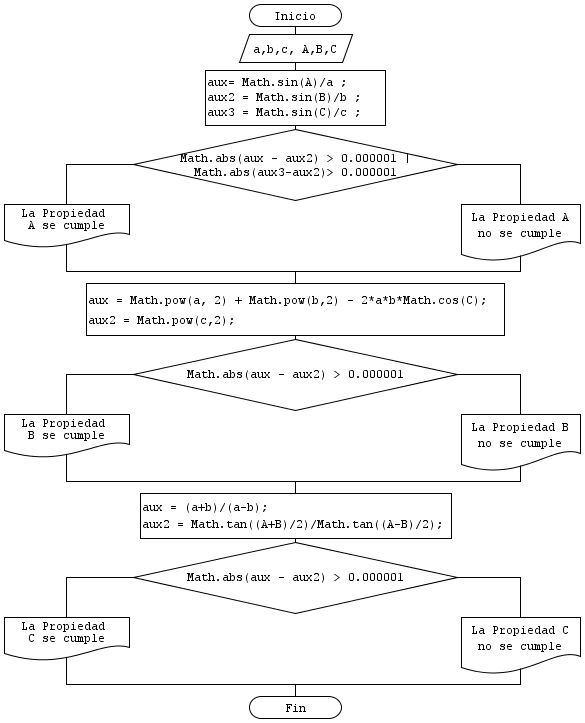
\includegraphics[scale=0.80]{dicor/Verifica.png}    
\end{figure}

\textit{Código en Java:}
\lstinputlisting[language = Java]{src/verificaLog.txt}
\newpage

\textbf{8. Ecuación.} Dados los valores de una ecuación cuadrática ax2 + bx + c = 0 hallar sus dos
raíces. Los valores a, b, c se ingresan por teclado y son números enteros. En el caso de
raíces imaginarias imprima el mensaje "no hay soluciónn en los números reales".
\textit{Diagrama de Flujo:  }
\begin{figure}[h!]
\centering
	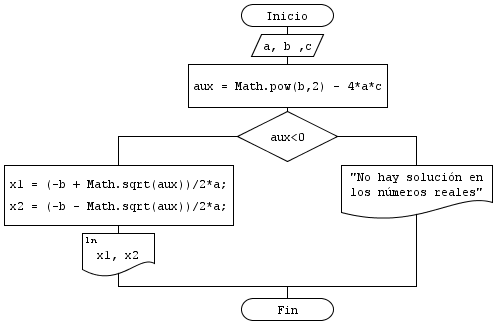
\includegraphics[scale=0.80]{dicor/Ecuacion.png}    
\end{figure}

\textit{Código en Java:}
\lstinputlisting[language = Java]{src/Ecuacion.txt}
\newpage

\textbf{9.  Romanos.} Escriba un programa que lea un número entero n (1 <= n <= 100), e imprima su
equivalente en número romano.

\textit{Diagrama de Flujo:  }
\begin{figure}[h!]
\centering
	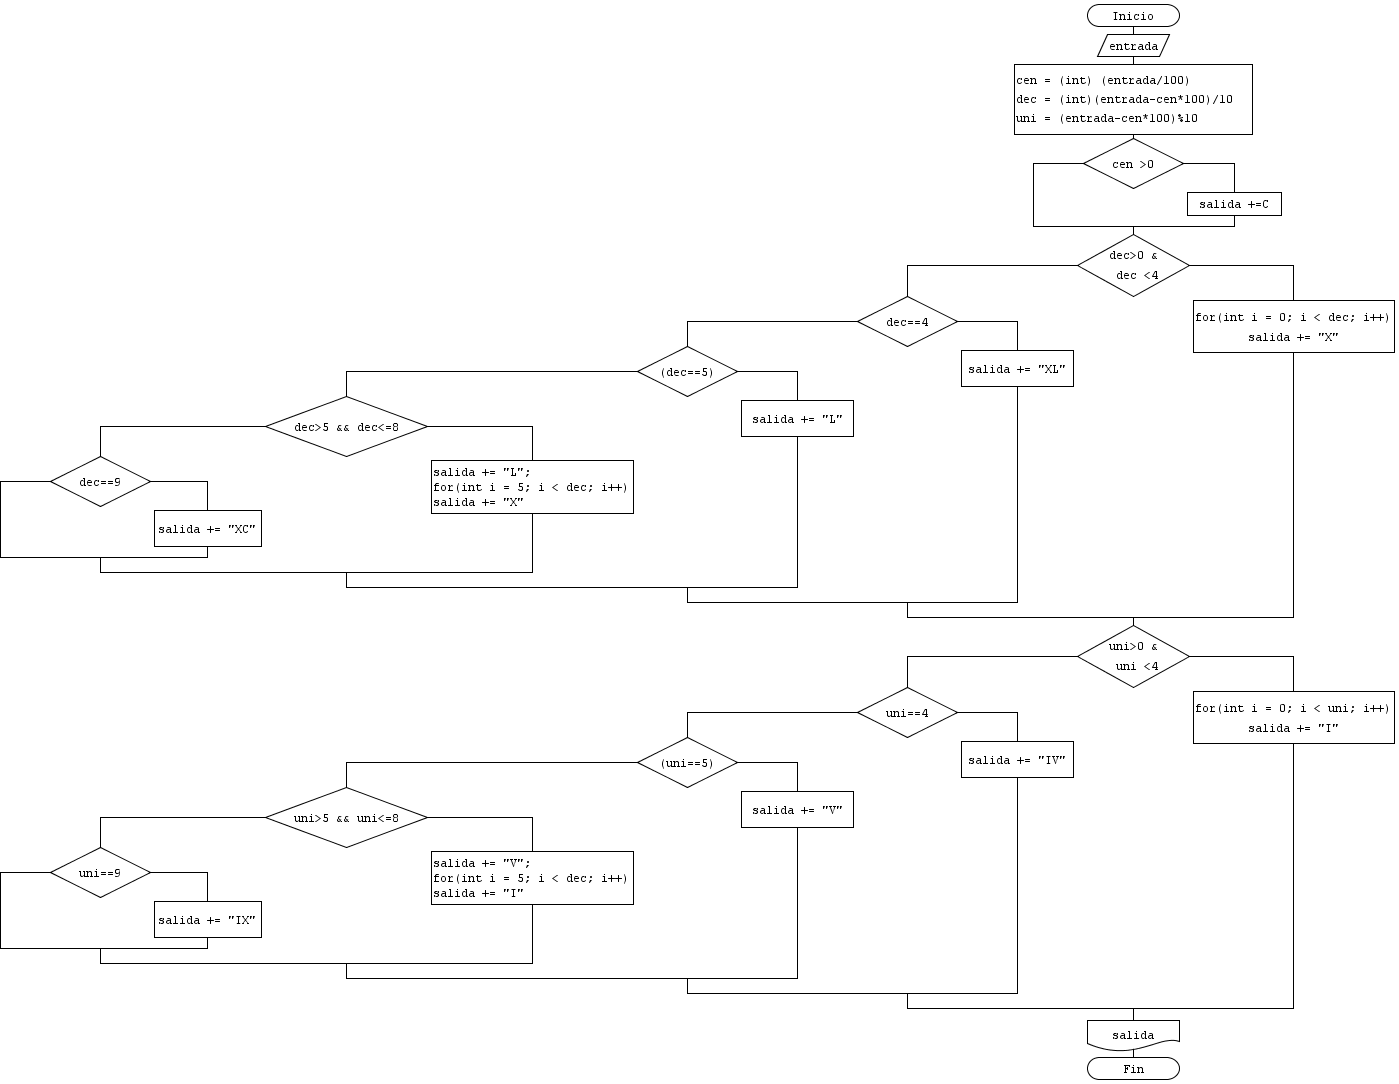
\includegraphics[scale=0.35]{dicor/Romanos.png}    
\end{figure}

\textit{Código en Java:}
\lstinputlisting[language = Java]{src/Romanos.txt}
\newpage


\textbf{10. Área de un Triángulo. } Escriba un diagrama que solicite ingresar 3 puntos del tipo\\
  x1, y1 \\
  x2, y2 \\
  x3, y3\\
 de un triángulo e imprima su área
 
\textit{Diagrama de Flujo:  }
\begin{figure}[h!]
\centering
	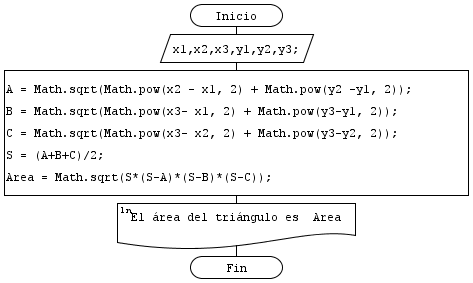
\includegraphics[scale=1]{dicor/AreaDeUnTriangulo.png}    
\end{figure}

\textit{Código en Java:}
\lstinputlisting[language = Java]{src/AreaDeUnTriangulo.txt}
\newpage


\textbf{11. Un ISBN-10} (Número de libro estándar internacional) consta
de 10 dígitos: d1,d2,d3,d4 ,d5,d6, d7 ,d8,d9,d10. El último dígito, d10, es una suma de comprobación, que se calcula a partir de los otros nueve dígitos
Si la suma de comprobación es 10, el último dígito se denota como X de acuerdo con la
convención ISBN-10. Escriba un programa que solicite al usuario ingresar los primeros 9
dígitos y muestre el ISBN de 10 dígitos (incluidos los ceros a la izquierda). Su programa
debe leer la entrada como un entero.

 
\textit{Diagrama de Flujo:  }
\begin{figure}[h!]
\centering
	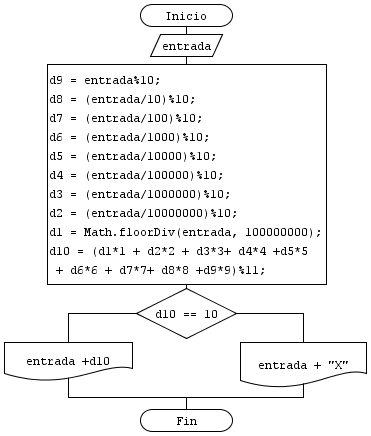
\includegraphics[scale=1]{dicor/ISBN.png}    
\end{figure}
\newpage
\textit{Código en Java:}
\lstinputlisting[language = Java]{src/VerificarElISBN.txt}
\newpage


\textbf{12. Ciencia:} día de la semana. La congruencia de Zeller es un algoritmo desarrollado por
Christian Zeller para calcular el día de la semana.\\
a) h es el día de la semana (0: sábado, 1: domingo, 2: lunes, 3: martes, 4: miércoles, 5:
jueves, 6: viernes).\\
b) q es el día del mes.\\
c) m es el mes (3: marzo, 4: abril, ..., 12: diciembre). Enero y febrero se cuentan como
los meses 13 y 14 del año anterior. \\
d) j es el siglo (es decir,año/100)\\
e) k es el año del siglo (es decir, año %100).\\
Tenga en cuenta que la división en la fórmula realiza una división entera. Escriba un
programa que solicite al usuario ingresar un año, mes y día del mes, y muestre el nombre
del día de la semana.

\textit{Diagrama de Flujo:  }
\begin{figure}[h!]
\centering
	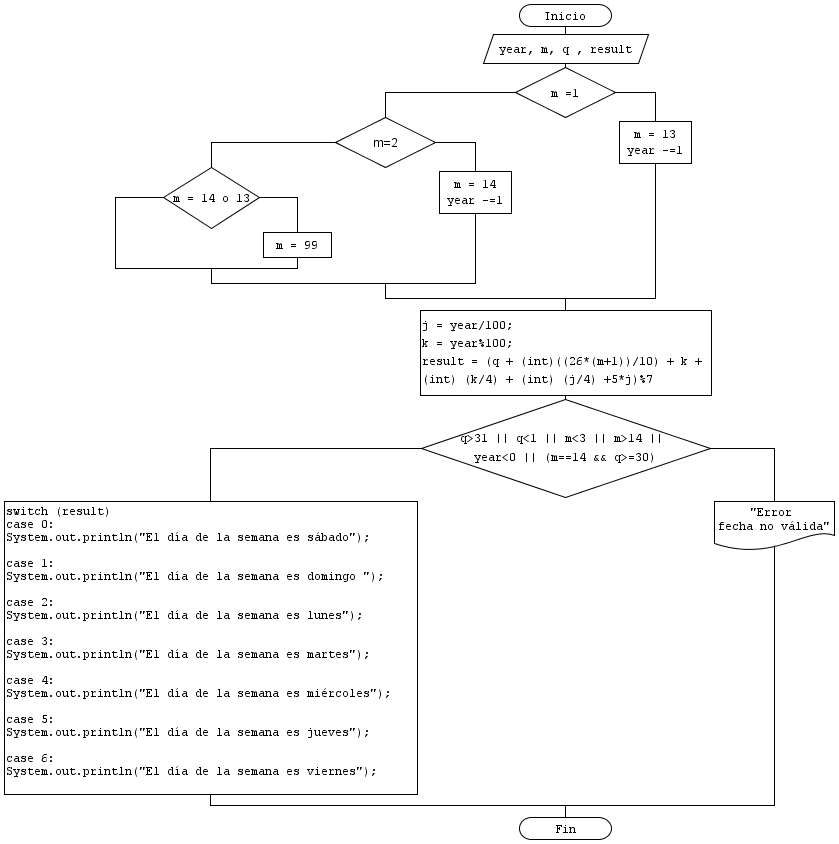
\includegraphics[scale=0.55]{dicor/DiaDeLaSemana.png}    
\end{figure}
\newpage
\textit{Código en Java:}
\lstinputlisting[language = Java]{src/DiaDeLaSemana.txt}
\newpage


\textbf{13.  Geometría:} >Apunté a un rectángulo? Escriba un programa que solicite al usuario ingresar
un punto (x, y) y verífique si el punto está dentro del rectángulo centrado en (0, 0) con
ancho 10 y alto 5. Por ejemplo , (2, 2) está dentro del rectángulo y (6, 4) está fuera del
rectángulo.  

\textit{Diagrama de Flujo:  }
\begin{figure}[h!]
\centering
	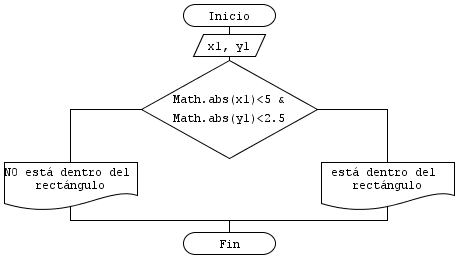
\includegraphics[scale=0.65]{dicor/GeometriaRectangulo.png}    
\end{figure}

\textit{Código en Java:}
\lstinputlisting[language = Java]{src/GeometriaRectangulo.txt}
\newpage
\end{document}

